\documentclass{article}
\usepackage[utf8]{inputenc}
\usepackage{amssymb}
\usepackage{amsfonts}
\usepackage{amsmath}
\usepackage[utf8]{inputenc}
\usepackage[norsk]{babel}
\usepackage{lmodern}
\usepackage{float}
\usepackage{graphicx}
\DeclareGraphicsExtensions{.pdf,.png,.jpg}
\usepackage{latexsym}
\usepackage{hyperref}
\usepackage[euler]{textgreek}
\usepackage{stackengine}
\usepackage[version-1-compatibility]{siunitx}
\usepackage{pdfpages}
\usepackage{fixltx2e}
\hypersetup{pdfborder={0 0 0}}
\usepackage{pgfplots}
\pgfplotsset{compat=newest}
\pgfplotsset{plot coordinates/math parser=false}
\newlength\figureheight
\newlength\figurewidth
\usepackage[section]{placeins}%Sørger for at plots og andre floats holder seg til sin section.
\setlength\parindent{0pt}%Setter indent til 0



\title{Exercise 3 - TTK4130 Modeling and Simulation}
\author{Camilla Sterud}
\date{}

\begin{document}

\maketitle

\newpage

\section{Problem 1}

\begin{equation*}
    \ddot x + c\dot x + g(1-(\frac{1}{x})^{\kappa}) = 0, \quad \kappa = 1.40, \: g = 9.81.
\end{equation*}



\subsection{a}
The system on state-space form:

\begin{align*}
    \underline{\underline{\dot x_1 = x_2}}\\
    \underline{\underline{\dot x_2 = g(x_1^{-\kappa} - 1) - cx_2}}
\end{align*}

\subsection{b}

Assume $x_1(t_0), x_2(t_0)$ known.

\begin{align*}
    \underline{\underline{x_{1, n+1} = x_{1,n} + h x_{2,n}}}\\
    \underline{\underline{x_{2, n+1} = x_{2,n} + h(g(x_{1,n}^{-\kappa} - 1) - cx_{2,n})}}
\end{align*}

\subsection{c}

\begin{equation*}
    \underline{\underline{\mathbf{k_1} = \begin{bmatrix}
    k_{11}\\
    k_{12}
    \end{bmatrix} = \begin{bmatrix}
        x_{1,n} \\
        g(x_{1,n}^{-\kappa} - 1) - cx_{2,n}
    \end{bmatrix}}}
\end{equation*}

\begin{equation*}
    \underline{\underline{\mathbf{k_2} = \begin{bmatrix}
    k_{21}\\
    k_{22}
    \end{bmatrix} = \begin{bmatrix}
        x_{2,n} + \frac{h}{2}k_{12}\\
        g((x_{1,n} + \frac{h}{2}k_{11})^{-\kappa} - 1) - c(x_{2,n} + \frac{h}{2}k_{12})
    \end{bmatrix}}}
\end{equation*}

\begin{align*}
    \underline{\underline{x_{1, n+1} = x_{1,n} + h k_{21}}}\\
    \underline{\underline{x_{2, n+1} = x_{2,n} + hk_{22}}}
\end{align*}

\subsection{d}

For $x = 1 = x_1 $, $\dot x_1 = x_2 = \dot x_2 = 0$. When inserted into the state space model this gives us $0 = g(x_1^{-\kappa} - 1)$, which is correct around $x_1 = 1$. This showes that $x_1 = 1$ is, in fact, a stationairy point. 
Setting $\dot x_1 = f_1$ and $\dot x_2 = f_2$, we can linearize about this point using:

\begin{equation*}
\Delta\dot x_1 = \left. \frac{\partial f_1}{\partial x_1} \right.\Bigg|_{\shortstack{\tiny $x_1 = 1$ \\ \tiny $\dot x_2 = 0$}} \Delta  x_1  + \left. \frac{\partial f_1}{\partial x_2} \right.\Bigg|_{\shortstack{\tiny $x_1 = 1$ \\ \tiny $\dot x_2 = 0$}} \Delta  x_2,
\end{equation*}

\begin{equation*}
\Delta\dot x_2 = \left. \frac{\partial f_2}{\partial x_1} \right.\Bigg|_{\shortstack{\tiny $x_1 = 1$ \\ \tiny $\dot x_2 = 0$}} \Delta  x_1  + \left. \frac{\partial f_2}{\partial x_2} \right.\Bigg|_{\shortstack{\tiny $x_1 = 1$ \\ \tiny $\dot x_2 = 0$}} \Delta  x_2.
\end{equation*}

This leaves us with the linearization.

\begin{equation*}
    \underline{\underline{\Delta \dot x_1 = \Delta x_2}}
\end{equation*}



\begin{equation*}
     \underline{\underline{\Delta \dot x_2 = -\kappa g \Delta x_1 - c \Delta x_2}}
\end{equation*}

\subsection{e}
After being linearized, the system can be writtes as

\begin{equation*}
    \Delta\dot x = \mathbf{A}\Delta x = \begin{bmatrix}
        0 & 1 \\
        -\kappa g & -c
    \end{bmatrix} \Delta x.
\end{equation*}

Setting up Euler's method for this we get 

\begin{equation*}
    \Delta x_{n+1} = (\mathbf{I} + h\mathbf{A})\Delta x_n.
\end{equation*}

This will be stable if $|\mathbf{I} + h\mathbf{A}| \leq 1$.

\begin{equation*}
    \bigg|\begin{bmatrix}
        1 & h \\
        -\kappa g h & 1-hc
    \end{bmatrix}\bigg| = 1 - hc + \kappa g h^2 \leq 1
\end{equation*}

In the first case, $c = 0$, this will never be stable, as it requires $h = 0$. With $c = 2\sqrt{g\kappa}$ the method is stable for any $\underline{\underline{h \leq \frac{2}{\sqrt{g\kappa}}}}$.

\section{Problem 2}

\begin{equation*}
    L\frac{di}{dt} + Ri = u, \quad t > 0, \: i(0) = i_0.
\end{equation*}

\subsection{a}

The enery stored in the circuit is equal to the enery stored in the inductor. This means that the storage funtion for this system is 

\begin{equation*}
    V = \frac{1}{2} L i^2 \Rightarrow \dot V = Li\frac{di}{dt} = iu - Ri^2.
\end{equation*}

The storage function is monotonically decreasing for $u = 0$, which means that the energy stored in the system will end up being zero. The energy can only be zero if the current is zero (given by the equation for the energy stored in an inductor), so the system is clearly asymptotically stable for $u = 0$ (it is in fact stable for all $u < \infty$). 

I don't have time to sketch this right now, but the current will always decrease to zero for $u = 0$.

\subsection{b}

$e(t) = i(t) - i_{ref}$, $\dot e = \frac{1}{L}(u - Ri)$. 

\begin{equation*}
    E(t) = \frac{1}{2}Le^2(t) \Rightarrow \dot E(t) = Le\dot e = ue - Rie.
\end{equation*} 

$\lim_{t\to \infty} \dot E (t) = 0$, since $E$ must be constant if $i$ is constant. $\lim_{t\to \infty} e(u - Ri) \Rightarrow \underline{\underline{u = Ri_{ref}}}$.

\subsection{c}

\begin{figure}[!ht]
    \centering
    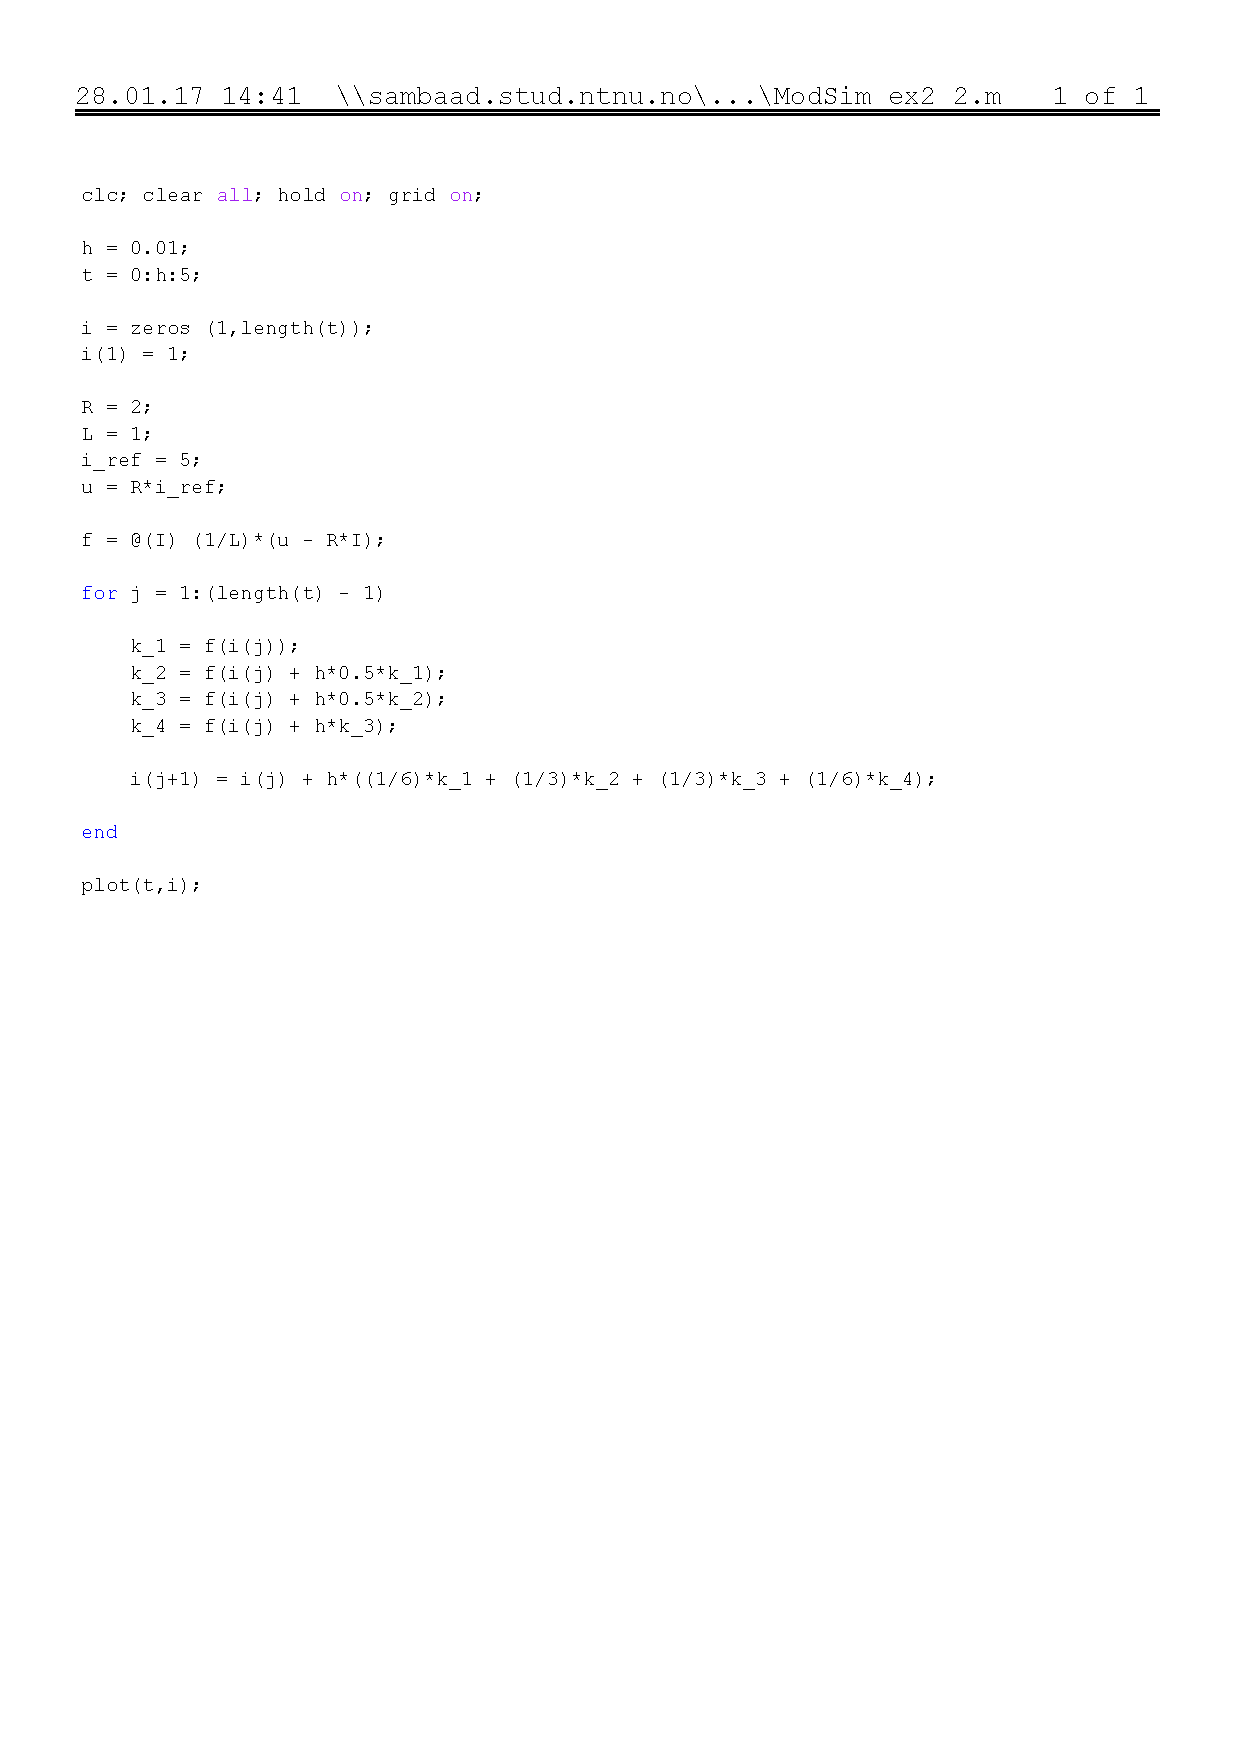
\includegraphics[width = \textwidth]{ex2_2_RK4}
    \caption{Code for solving the system with Explicit Runge-Kutta of order 4 in MATLAB.}
    \label{fig:matlabcode} 
\end{figure}

\subsection{d}

\begin{figure}[!ht]
    \centering
    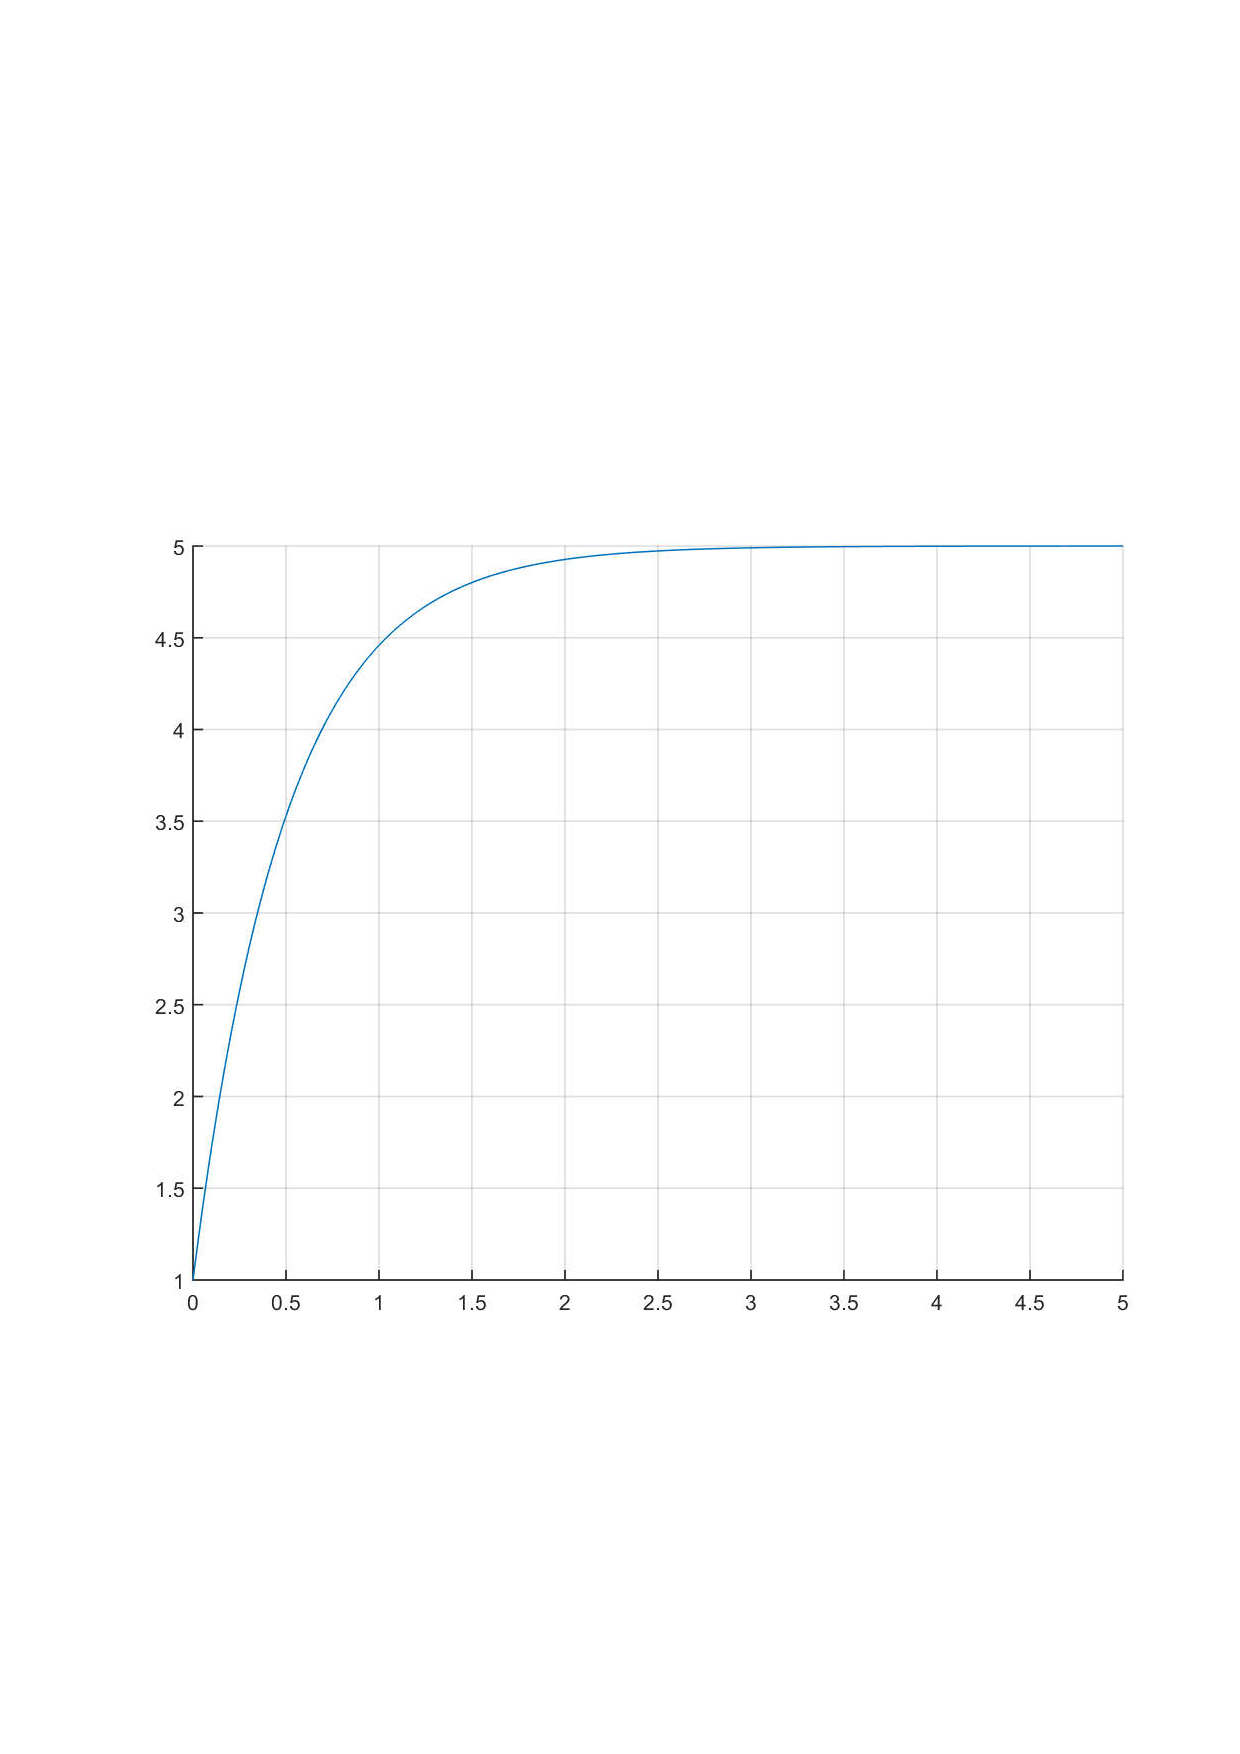
\includegraphics[width = 0.5\textwidth]{ex2_2_RK4_plot}
    \caption{The system solved with the MATLAB code.}
    \label{fig:RK4MATLAB} 
\end{figure}

\begin{figure}[!ht]
    \centering
    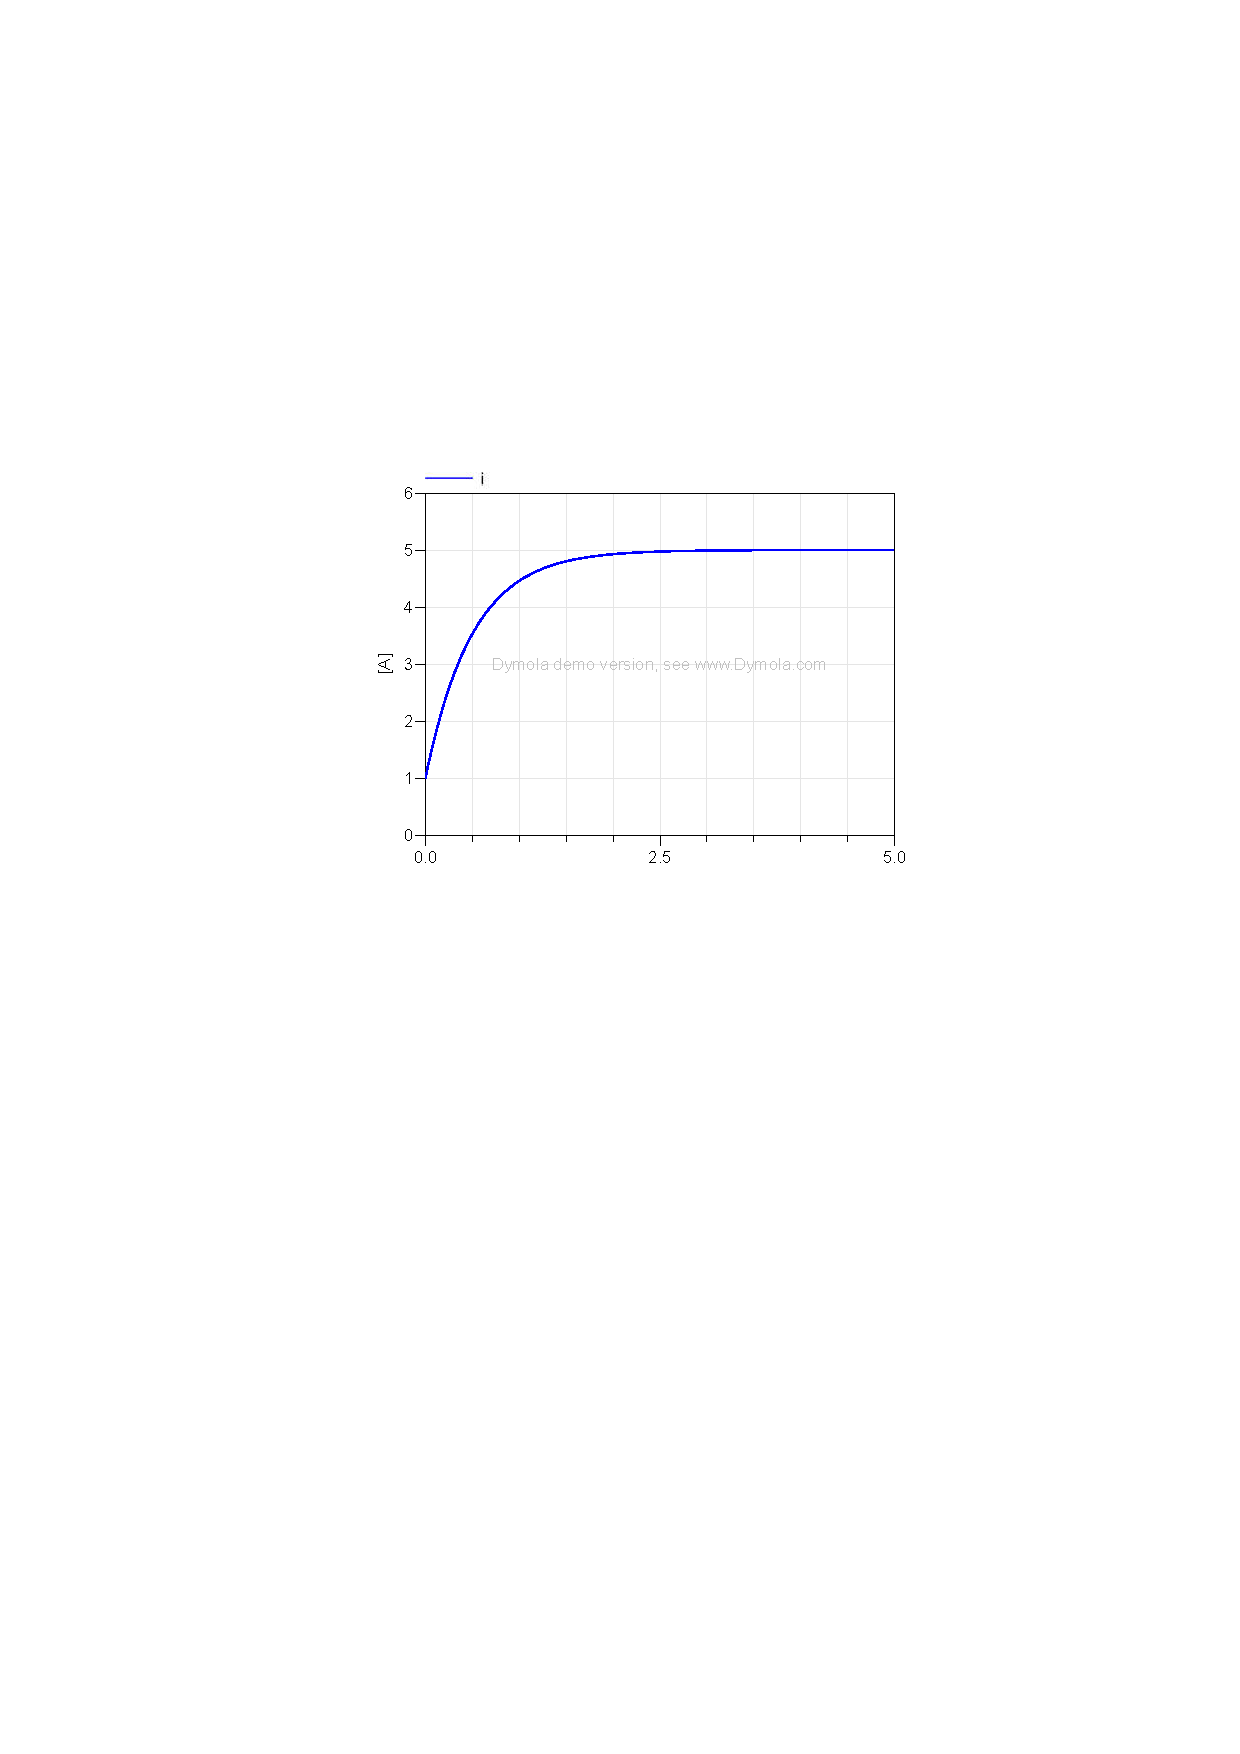
\includegraphics[width = 0.5\textwidth]{ex2_2d}
    \caption{The system solved with RK4 in Dymola.}
    \label{fig:RK4Dymola} 
\end{figure}

The MATLAB and Dymola plots look suspiciously alike.

\section{Problem 3}

\subsection{a}

\begin{figure}[!ht]
    \centering
    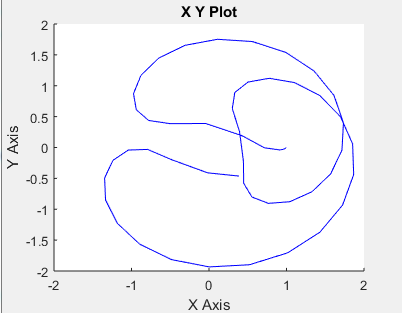
\includegraphics[width = 0.5\textwidth]{r1_rt_e1}
    \caption{1 round, Relative Tolerance (RT) = 10.}
\end{figure}

\begin{figure}[!ht]
    \centering
    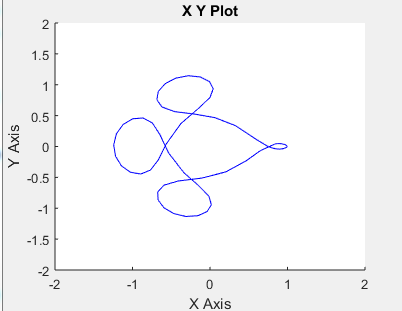
\includegraphics[width = 0.5\textwidth]{r1_rt_e-2}
    \caption{1 round, RT = 0.01. This works.}
\end{figure}

\begin{figure}[!ht]
    \centering
    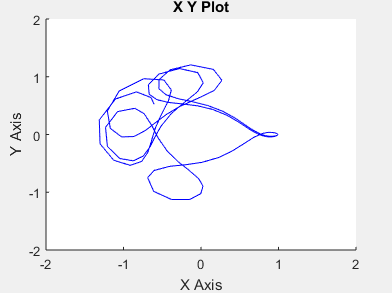
\includegraphics[width = 0.5\textwidth]{r2_rt_e-4}
    \caption{2 rounds, RT = 0.0001.}
\end{figure}

\begin{figure}[!ht]
    \centering
    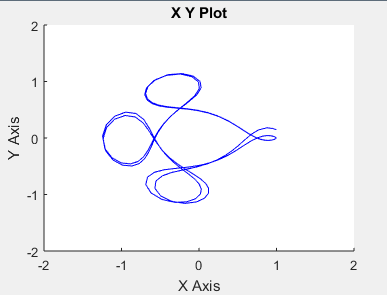
\includegraphics[width = 0.5\textwidth]{r2_rt_e-5}
    \caption{2 rounds, RT = 0.00001. This works.}
\end{figure}

\begin{figure}[!ht]
    \centering
    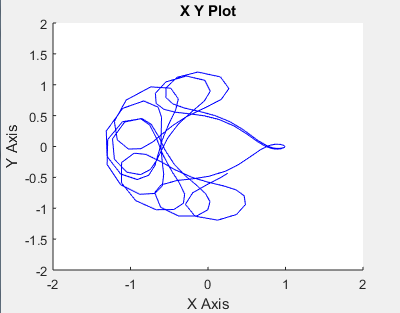
\includegraphics[width = 0.5\textwidth]{r3_rt_e-4}
    \caption{2 rounds, RT = 0.00001. } 
\end{figure}

\begin{figure}[!ht]
    \centering
    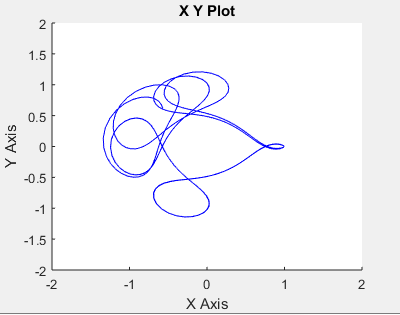
\includegraphics[width = 0.5\textwidth]{r3_rt_e-7}
    \caption{2 rounds, RT = $1e-7$. This works, kinda.}
\end{figure}

\subsection{b}

\begin{figure}[!ht]
    \centering
    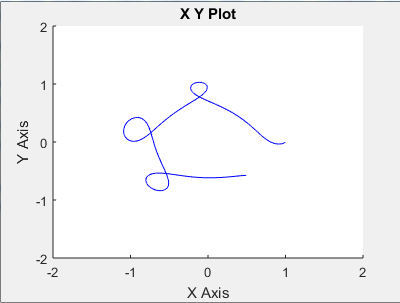
\includegraphics[width = 0.5\textwidth]{step_005}
    \caption{1 round with ode5 solver. h = 0.005.}
\end{figure}

\begin{figure}[!ht]
    \centering
    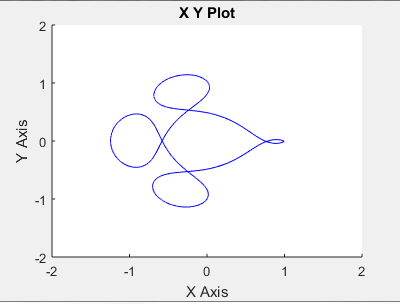
\includegraphics[width = 0.5\textwidth]{step_0025}
    \caption{1 round with ode5 solver. h = 0.0025. It's ok.}
\end{figure}



\end{document}